\chapter{Conclusion}
\label{chap:conclusion}
This thesis had two key objectives: (1) {explore the use of radar for gesture recognition} and (2) {provide tools and methods to facilitate the development of highly usable (radar-based) gesture interfaces}.
%
This chapter concludes our thesis in two sections.
Section~\ref{sec:conclusion:summary} summarizes our findings and contributions, and Section~\ref{sec:conclusion:limitations-and-future-works} discusses potential avenues for future research.


%================================================================================%
\section{Summary}
\label{sec:conclusion:summary}
In this section, we summarize the findings and contributions from the six main chapters of this thesis.

% State of the art
\subsubsection{Chapter~\ref{chap:state_of_the_art}: State of the Art}
This chapter explored the state of the art of gesture recognition through targeted and systematic literature reviews.

We first conducted a TLR to gain a general understanding of gesture-based interaction. 
%
We recognized the efficacy of GESs for involving end users in the development of highly usable gesture-based applications, as user-elicited gestures with high agreement have been associated with higher memorability~\cite{Vatavu:2014b}.
%
We also identified the key challenges of gesture interaction and potential solutions. These challenges included sensor limitations, jitter caused by tracking errors, noise, or hand tremors, intra- and inter-user variability of gesture production, gesture segmentation, and overlapping gestures. Effectively addressing these challenges while factoring in user preferences requires a high level of expertise in UX design, gesture recognition, and application development.
%
This high entry barrier and the lack of accessible tools for developers might explain why we identified relatively few gesture-based applications in the literature, despite their broad appeal across many facets of society. 

We then carried out an SLR on LMC-based gesture recognition. This choice to analyze a relatively mature vision-based technology like the LMC aimed to provide insights for contextualizing the current state of the research in radar-based gesture interaction.
%
We observed that, despite the popularity and ease of use of the LMC, none of the papers identified in the SLR proposed an approach that was reusable across gesture sets, gestural UIs, and applications. On the contrary, a large proportion of these papers resorted to opportunistic techniques for gesture recognition, such as hard-coded thresholds and sensor-specific gestures, which are difficult to maintain and lack portability.

With this context in mind, we undertook a second SLR to gain a comprehensive understanding of the current state of research in radar-based gesture interaction. We noticed that most of the research focused on radar systems, signal processing techniques, and algorithms for gesture recognition, with only a handful of papers demonstrating potential use cases of their systems with prototype applications. 
%
In addition, the scarcity of publicly available datasets in these papers hinders collaboration among researchers, while the plethora of sensors used, often custom-designed, and the reliance on deep learning algorithms for gesture recognition, makes it difficult to apply these results to a different environment.

Finally, we concluded this chapter by positioning our work within the existing literature in the light of our findings.

% QuantumLeap 
\subsubsection{Chapter~\ref{chap:quantumleap}: Facilitating the Development of Gesture-based Applications}
This chapter introduced \ql, a modular framework designed to bridge the gap between researchers and practitioners to foster the development of gesture-based applications.

Its modular architecture encapsulates all of the gesture recognition logic and only exposes a simple API to the application, which allows developers to map gestures to actions without focusing on acquiring, segmenting, and recognizing gestures. The configuration GUI of \ql makes it easy for developers to set up the gesture recognition dataflow for their needs without having to modify its source code. Additionally, its modular architecture facilitates future updates to the dataflow, such as an improved gesture recognizer or a new gesture set.

We evaluated the framework among seven developers with varying levels of expertise, which resulted in a good usability rating. Despite the limitations of this study, such as the excessive guidance provided to the participants, it offered valuable insights for future improvements to \ql. 
%
They include providing more guidance to users when configuring the dataflow (\eg module recommendations) and addressing the rigidity of the \ql dataflow architecture to support more complex gesture recognition techniques.

Despite these limitations, the \ql framework was used by many students over the years, who contributed to the project by implementing new modules and developing unique gesture-based applications.

% QuantumLeap Testing
\subsubsection{Chapter~\ref{chap:quantumleap-testing}: Streamlining the Evaluation of Gesture Recognizers}
This chapter introduced the \ql testing tool, an extension of \ql designed for evaluating the performance of gesture recognizers. 

The tool relies on the same modules and datasets as \ql and supports ten distinct testing procedures. In addition, its testing configurations and results can be exported in a standardized format, which is extremely convenient as researchers can now easily share all of the elements required to attempt to repeat, replicate, and reproduce their results.

The tool inherits some of the limitations of \ql, including its relatively rigid architecture, which complicates the evaluation of more complex gesture recognition pipelines.
Despite its limitations, it has been used extensively in the rest of the thesis.

% LUI
\subsubsection{Chapter~\ref{chap:lui}: Designing Highly Usable Gesture-based Applications}
This chapter proposed a user-centered iterative development method and evaluation protocol for gesture-based applications, designed to facilitate the creation of highly usable gestural interfaces. 

The proposed method comprises three key steps. 
%
First, a consistent set of gestures is designed, incorporating user preferences derived from the literature or a GES.
%
Then, a gesture recognition dataflow is implemented, \eg utilizing our \ql framework. An optimal dataflow configuration may be identified through a benchmarking of gesture recognizers on the selected gesture set.
%
Finally, an experiment is conducted to assess the usability of the resulting application. Depending on the experiment's outcome, a new iteration of this process may be started to improve the application based on these new insights.

We successfully applied this method to \lui, a gesture-based application for browsing and manipulating multimedia content, such as images, videos, documents, and maps. 
%
Implementing gesture recognition through \ql proved instrumental in supporting complex gestures with relatively low effort, such as the manipulation of multimedia objects with immediate and continuous feedback. In addition, the separation of concerns provided by the framework enables users to customize the gesture set of \lui without having to delve into its source code.
%
Finally, the consistent set of gestures featured in \lui resulted in a relatively effective and usable interface, as indicated by our usability evaluation conducted among 17 participants. Some limitations were also highlighted, including an unpredictability in gesture recognition for certain gestures, attributed in part to slight variations in the way they were performed by the participants. This emphasizes the importance of supporting user-defined gestures.

% RadarSense
\subsubsection{Chapter~\ref{chap:radar-challenges}: Addressing the Challenges of Radar-based Gesture Recognition}
This chapter introduced a full-wave electromagnetic model and inversion-based~\cite{Lambot:2004,Lambot:2014} radar signal processing pipeline, aimed at addressing some of the challenges of radar-based gesture recognition. In particular, the variance between radar systems and their sensitivity to objects in the environment.

% 6 stages of the pipeline
The pipeline consists of six stages: (1) raw data capture, (2) radar source and antenna effects removal, to remove internal reflections and transmissions between antennas, as well as antenna-target interactions, (3) background scene removal, to remove the reflections of static objects in the vicinity of the radar, (4) time gating, to ignore remaining reflections from objects situated past a certain distance from the radar, such as people moving behind the user, (5) full-wave inversion, to reduce the radar signal to only two physically-meaningful metrics (distance and permittivity), and (6) filtering, to smooth out errors in the inversion process and discard unrealistic values.

Two small experiments were conducted to (1) analyze whether the pipeline could effectively normalize signals from two distinct radars, and (2) investigate the sensitivity of our pipeline to variations in radar-target distance and angle.
%
Although the results of our first experiment were conclusive, the second experiment showed that signals from our processing pipeline changed with both radar-target distance and angle.  

% Implementation + application
Different implementations of the pipeline were provided for batch and real-time signal processing, and a prototype application was created to demonstrate potential use cases of the pipeline.


% Radar experiments
\subsubsection{Chapter~\ref{chap:radar-experiments}: Experimenting with Radar-based Gestures}
This chapter investigated the efficacy of our radar signal processing pipeline in three experiments.

% First experiment
The first experiment compared the performance of three different sensors (an LMC, a custom radar, and a Walabot) on a dataset of 16 gestures. Its results revealed that the Walabot could achieve better accuracy than the LMC and the custom radar, suggesting that inexpensive antenna arrays could be used successfully for gesture interaction.

% Second experiment
The second experiment evaluated the Walabot in user-dependent, user-independent, and mixed scenarios on an extended dataset of 20 gestures and well-differentiated subsets of gestures. The results suggested that employing smaller, well-differentiated sets of gestures, coupled with supporting user-defined gestures, could be the key to building reliable radar-based gesture recognition. 

% Third experiment
The third experiment analyzed the impact of occlusion by three different types of materials (wood, PVC, and glass) on a dataset of nine gestures. It showed that our pipeline could successfully normalize radar signals, provided that the signal-to-noise ratio was high enough. Indeed, the system still achieved high accuracy when obstructed by materials with a low relative permittivity like wood and PVC.

% Discussion
We drew ten implications for radar-based gesture recognition from our experiments, which we categorized into four key areas. 
%
The first implication relates to the radar systems, recommending the use of multiple spatially separated radar antennas when possible.
%
Several implications address gesture sets, in particular, how they can be designed to maximize gesture recognition accuracy. They underscore the importance of collecting gestures from a wide range of users and supporting user-defined gestures. They also suggest favoring gestures with motion parallel to the radar beam and with highly differentiable surfaces of exposure.
%
Two implications relate to the signal processing pipeline, advising developers to carefully select the necessary stages of the pipeline for their specific needs and suggesting the use of time-domain data instead of frequency-domain.
%
The last two implications consider the environment of interaction, cautioning against the use of materials with high relative permittivity and stressing the importance of performing gestures within the appropriate range of the radar.
%
These implications can serve as a valuable guide for developers when designing radar-based gestural interfaces. 

% %================================================================================%
% \section{Contributions}
% \label{sec:conclusion:contributions}
% In this section, we review our main contributions in the light of the four ISO/IEC 25010 software quality properties~\cite{iso25010} mentioned in the introduction (Section~\ref{sec:introduction:research:research-questions}): compatibility, maintainability, portability, and usability.

% \subsubsection{Literature Reviews}
% We conducted one TLR and two SLRs to gather insight into the state of research in the field of (radar-based) gesture interaction.
% %

% Our TLR on gestural interaction 

% Our TLR and LMC SLR:
% Compatibility: /
% Maintainability: mostly non-reusable approaches, often opportunistic. Evolution depends on how sensor API is maintained and supporting other gestures may require substantial modifications to the source code.
% Portability: many of the discussed papers relied on opportunistic gesture recognition techniques that are often tied to the exact sensor used. Substantial work would be needed to adapt the applications and recognition techniques proposed by these papers to other sensors. 
% Usability: relatively high entry barriers for building highly usable gesture-based applications, as they require expertise in gesture recognition, UX design, and application development. Few tools exist

% RADAR SLR:
% Compatibility: very few datasets publicly available, techniques specific to one radar in particular
% Maintainability: many deep learning based approaches, which take time for re-training (new gesture set, environment...)
% Portability: many different radars, gesture recognition techniques that are tailored to one gesture set and radar
% Usability: few real applications, but a large part of the proposed techniques for gesture recognition do not support user-submitted gestures without extensive re-training, which can negatively impact usability~\cite{Nacenta:2013}.


% A targeted literature review (TLR)~\cite{Kysh:2013} and two systematic reviews of the literature (SLR)~\cite{Kitchenham:2010} were conducted to gather insight into the state of research in the field of (radar-based) gesture interaction:
% \begin{itemize}
%     \item \textit{TLR on gestural interaction}: a summary of the literature on the topic of gesture-based interaction in general, including gesture elicitation studies, the challenges of gesture recognition, and examples of gesture-based interfaces.
%     \item \textit{SLR on LMC-based gesture interaction}: a look into how the LMC, a relatively mature vision-based sensor for gesture interaction, was used by researchers and practitioners to implement gesture recognition.
%     \item \textit{SLR on radar-based gesture recognition}: a deep dive into the state of radar-based gesture recognition in the literature that focuses on applications, radar systems, gestures, and algorithms.
% \end{itemize}

% \subsubsection{Tools and Methods}
% We provide two tools and one method that aims at fostering the development of highly usable (radar-based) gesture interfaces:
% \begin{itemize}
%     \item \textit{\ql framework}: a tool that addresses most of the challenges usually faced when creating gestural interfaces and provides an easy way to evaluate and compare gesture recognition algorithms. Its modular architecture featuring standardized modules facilitates the sharing of algorithms, sensors, and datasets across researchers and practitioners.
%     \item \textit{User-centered development method}: an iterative development method and evaluation protocol for gestural interfaces that guide developers through the design process of highly usable gesture-based applications.
%     \item \textit{Radar data pre-processing pipeline}: an electromagnetic model and inversion-based approach that normalizes radar signal to become independent from the radar system and background scene.
% \end{itemize}

% QUANTUMLEAP:
% Compatibility: 
% - interoperability: standardized modules and datasets that are easy to share and reuse, in particular between \ql and its testing tool.
% - co-existence: the current version of \ql and its testing tool do not support the co-existence sub-property of compatibility, because running a benchmark pauses the gesture recognition dataflow and \ql does not support multiple applications simultaneously (\eg need to change config and restart to switch to another gesture-based application)

% Maintainability: modular architecture enables devs to change/improve a module without impacting the rest of the dataflow. Modules can be reused across applications and benchmarks. Separation of concerns enables devs to change the dataflow without having to modify the application UI. \ql testing tool enables testing the performance of algorithms before using them in an application

% Portability: \ql testing configurations, modules, and datasets can be shared with other developers so that they can easily compare their new algorithms in the same conditions as existing ones, thus helping advancing the state of literature.

% Usability: supports accessibility, by enabling users to use their own set of gestures. developers can focus on the quality of the UI instead of gesture recognition pipeline, which can result in more usable applications.


% USER DEVELOPMENT METHOD:
% Compatibility: /
% Maintainability: /
% Portability: /
% Usability: our methodology encourages developers to involve end users in the development process: GES to identify user preferences, evaluation with a panel of potential end users

% RADAR PROCESSING PIPELINE:
% Compatibility: provides some level of interoperability between radar systems by normalizing their radar signals. Datasets produced with one radar could thus be reused with another radar, provided that they operate at similar frequency ranges.
% Maintainability: similarly, one radar + gesture set can be used in another environment without having to re-record all gestures in the new environment thanks to data normalization. Just requires a re-calibration of the radar and/or a new snapshot of the background scene
% Portability: can adapt to different environments, including behind materials, different background scenes,... thanks to calibration and background scene removal stage. Can adapt to many different radar systems, which we illustrated with a custom radar equipped with a single horn antenna and an off-the-shelf Walabot Developer radar.
% Usability: contribute to more accurate gesture recognition + in the future, easier access to radar-based applications, as many radar systems may become compatible with each other.



% \subsubsection{Applications}
% We developed one gesture-based application in the context of this thesis, but many more were built by other developers using \ql (see Section~\ref{sec:quantumleap:integration}): 
% \begin{itemize}
%     \item \textit{Large User Interface}: a gesture-based application that enables the manipulation of multimedia content with hand gestures and serves as a demonstration of the \ql framework and our user-centered development method.
% \end{itemize}

% Illustrates the main properties of \ql and our development method in an application: (no need to go too in-depth)
% Compatibility: the configuration of \ql for \lui could be reused in another application
% Maintainability: easier to maintain thanks to the modular architecture of \ql and the separation of concerns.
% Portability: we could change the LMC sensor by another sensor without having to change the \lui source code. Just need to change \ql config with new dataset of gestures from the new sensor and new module for the sensor.
% Usability: resulted in relatively high usability (see experiment), users can propose their own gestures (however,  an interface for that could be integrated into the \lui application)

% \subsubsection{Datasets and Experiments}
% Three experiments were conducted, each with its corresponding dataset, to evaluate the performance of our radar data pre-processing pipeline on a wide range of gestures performed by multiple users in different contexts.
% These datasets allow the testing and comparison of gesture recognition techniques under various conditions and will thus be made publicly available to foster research and development in the field of gesture recognition.
% \begin{itemize}
%     \item \textit{Sensors comparison}: a dataset featuring 16 gesture classes from one participant recorded with three different devices, including two radars and an LMC. The corresponding experiment compares the performance of the three sensors in various testing configurations.
%     \item \textit{20 gestures}: a dataset featuring 20 gesture classes from six participants recording with a Walabot sensor. The corresponding experiment evaluates the suitability of radar sensors for recognizing large sets of gestures and identifies smaller subsets of highly-differentiable gestures.
%     \item \textit{Gestures through materials}: a dataset featuring nine gesture classes from 20 participants recorded with a Walabot through three types of materials (wood, PVC, and glass). The corresponding experiment investigates the performance of the Walabot when sensing gestures through materials and the ability of our pre-processing pipeline to normalize radar data sensed through different materials.
% \end{itemize}

% Compatibility: standardized gesture set format, that we make publicly available. As such, all our datasets can be used for testing and in gesture-based application with \ql, but also by other researchers if their tool supports our standardized format.
% Maintainability: our experimental protocol based on the \ql testing tool makes it easy to evaluate different recognizers on the same gesture sets, to apply our testing protocol to different gestures, or to adapt the testing protocol \textbf{TODO make configs and datasets available (urls)}
% Portability: thanks to \ql, or experiments can be reproduced by other researchers easily (to check if they can produce the same results in the same conditions) and replicated (to check if they get similar results in a different conditions (environment,...)).
% Usability: evaluating the performance of gesture recognizers is key to building highly usable gesture-based interfaces, as low recognition accuracy can result in frustration, confusion, and thus a lower usability.

%================================================================================%
\section{Future Works}
\label{sec:conclusion:limitations-and-future-works}
We envision three key avenues for future research to address the main limitations of this thesis.

\begin{figure}[htp]
  \centering
  \begin{subfigure}{\textwidth}
      \centering
      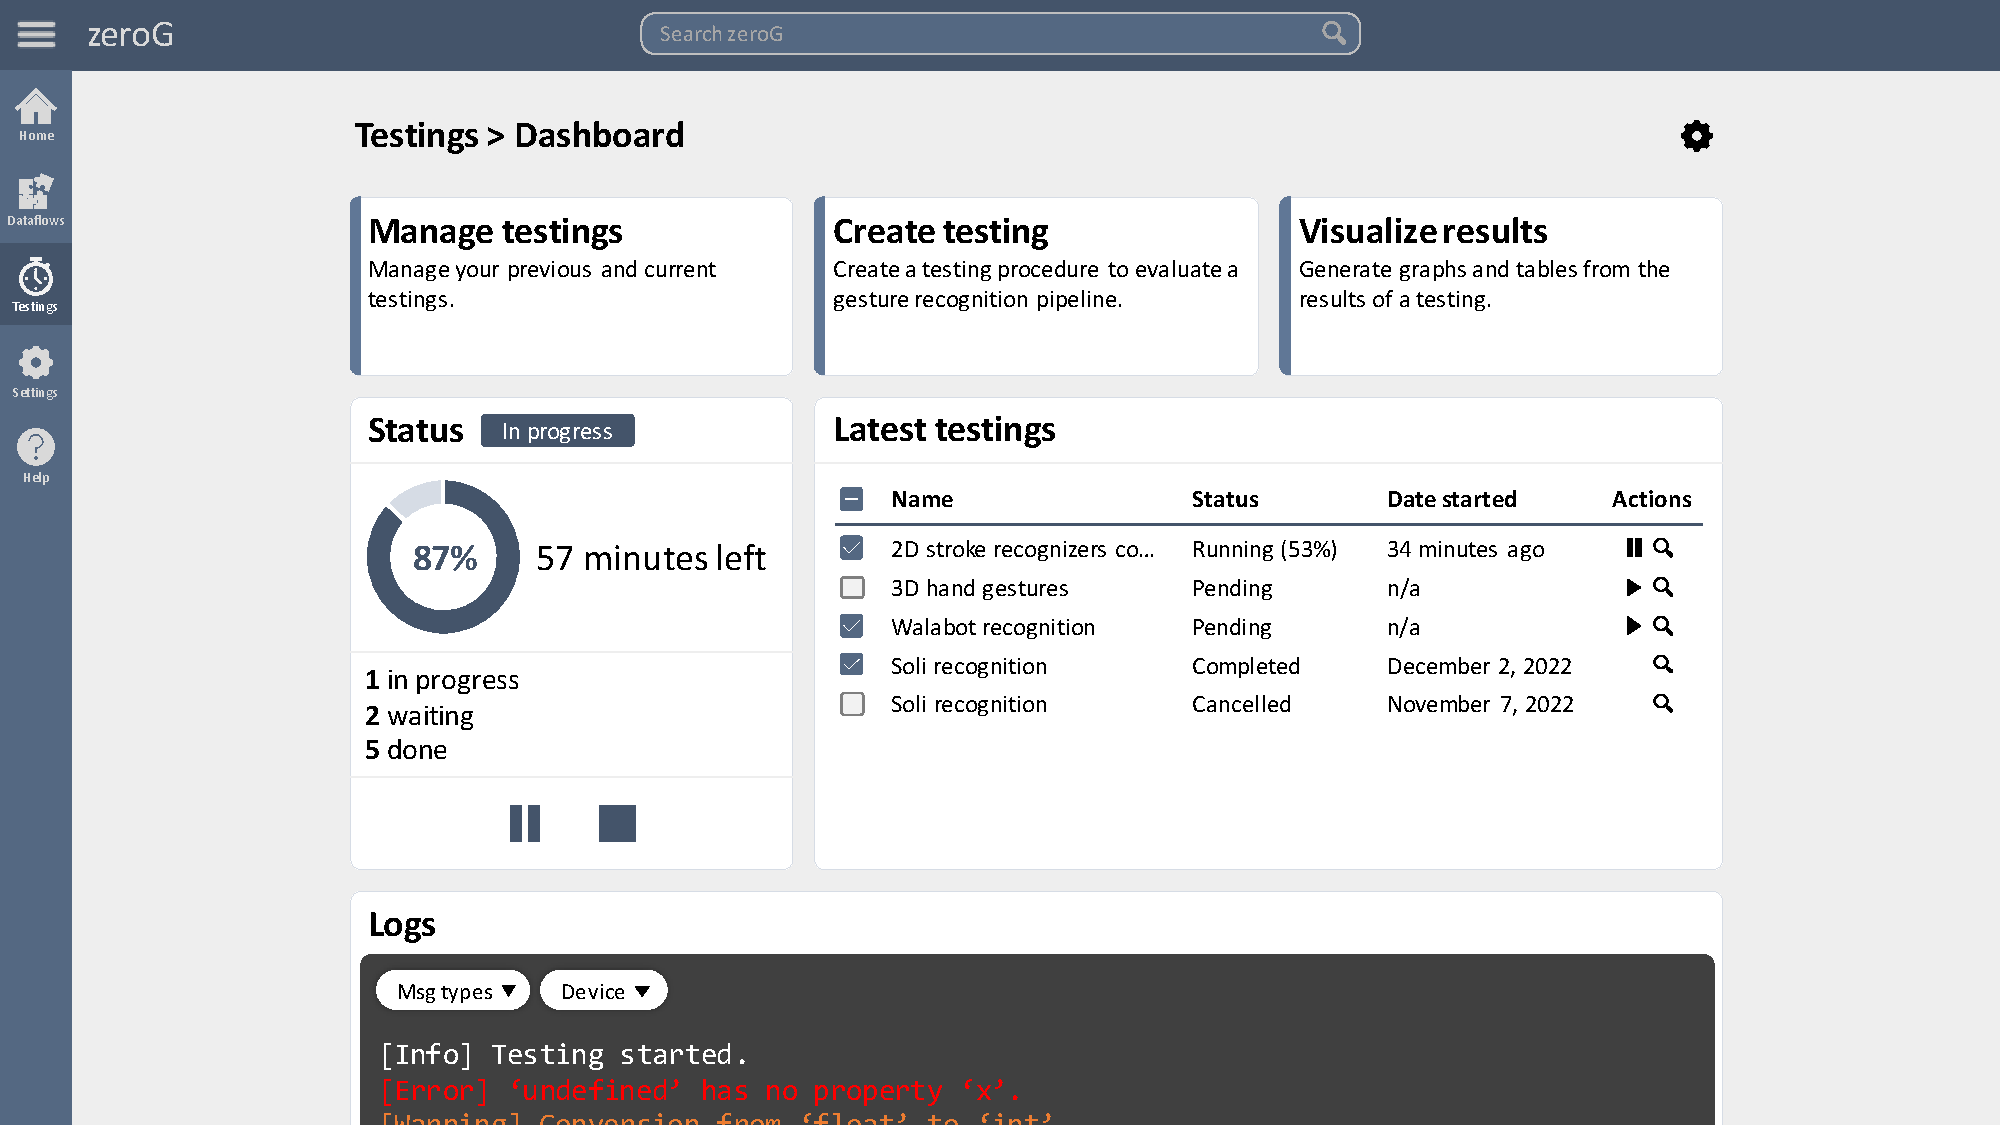
\includegraphics[width=.79\linewidth]{Figures/Conclusion/zeroG-1.pdf}  
      \vspace{-4pt}
      \captionsetup{width=.9\linewidth}
      \caption{Testing dashboard.}
      \label{fig:zerog:ui:1}
  \end{subfigure}

  \begin{subfigure}{\textwidth}
      \centering
      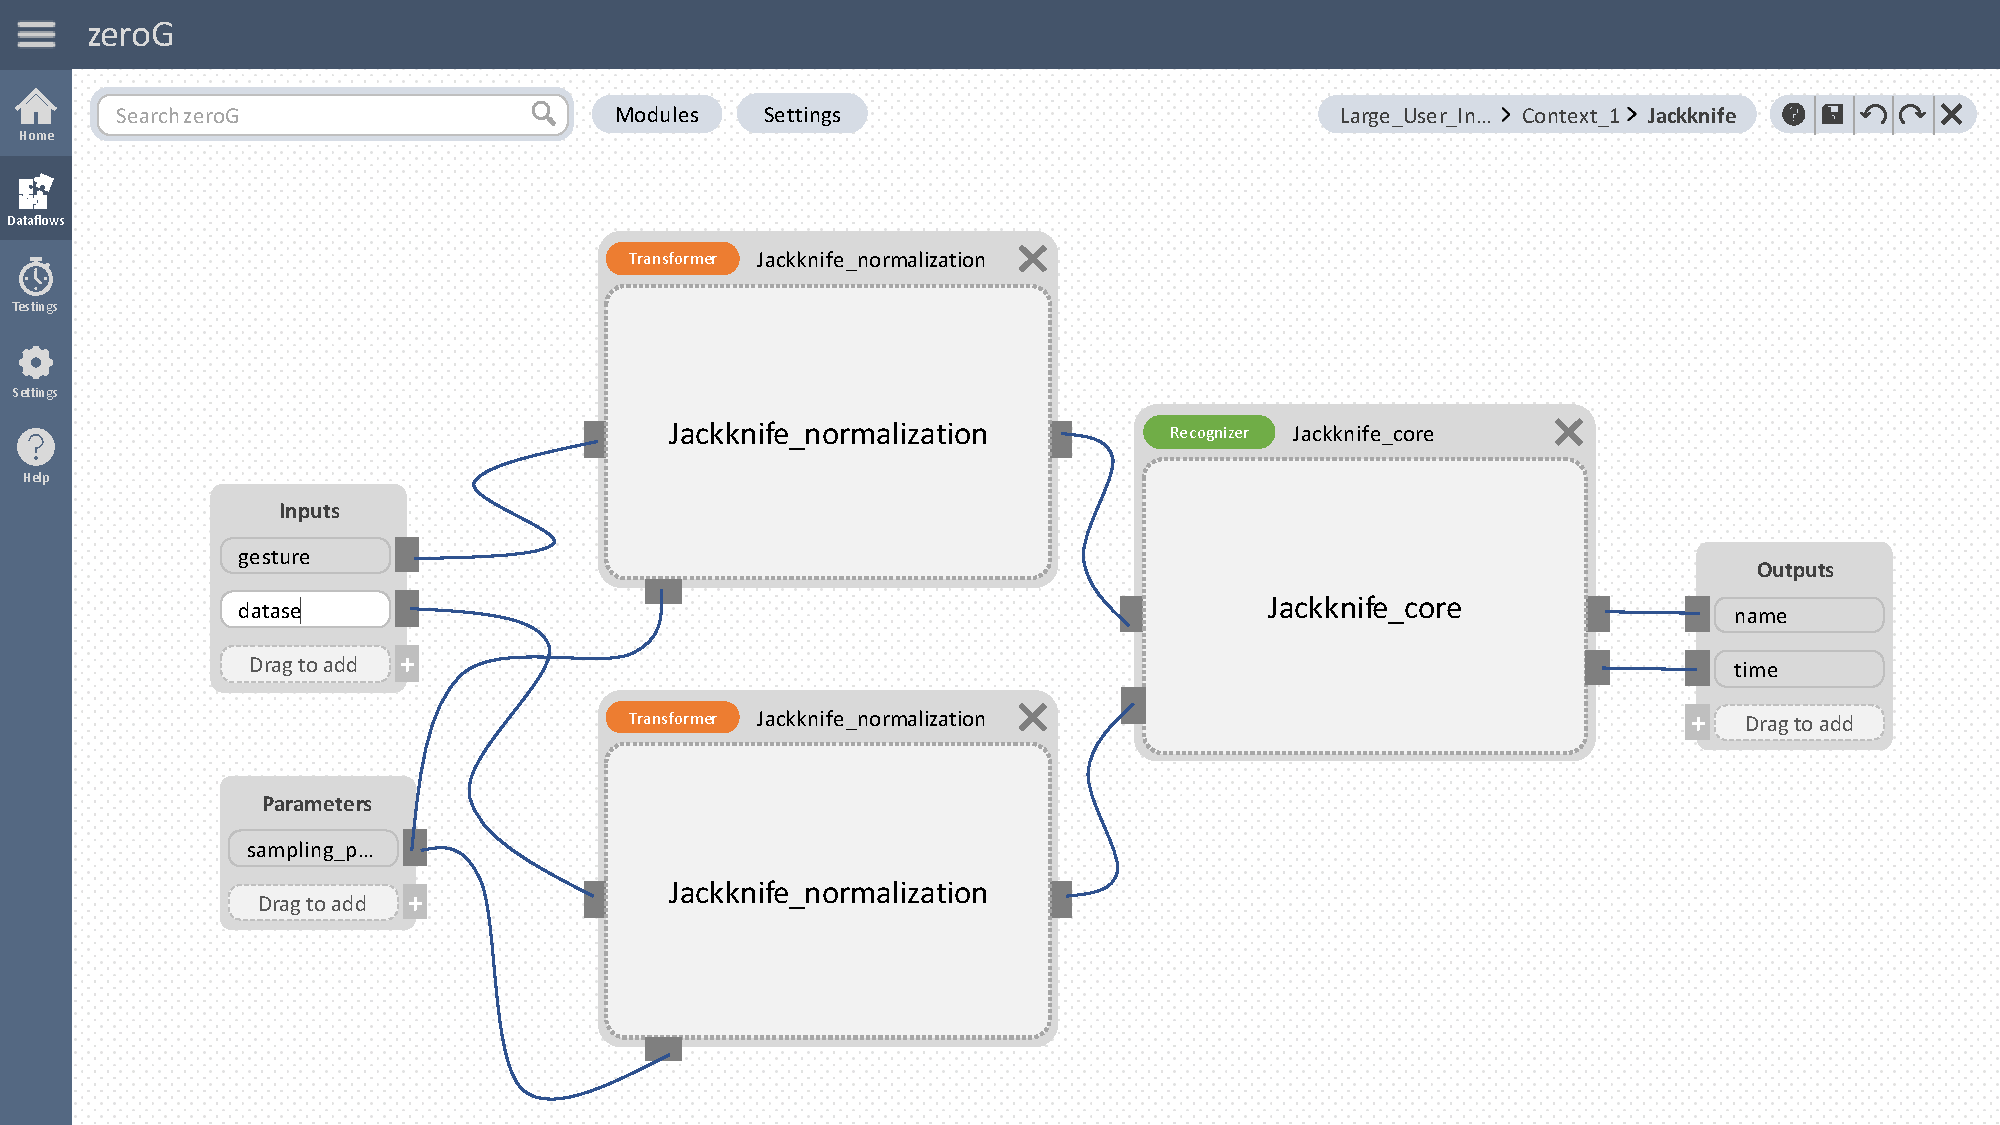
\includegraphics[width=.79\linewidth]{Figures/Conclusion/zeroG-2.pdf}  
      \vspace{-4pt}
      \captionsetup{width=.9\linewidth}
      \caption{Dataflow creation.}
      \label{fig:zerog:ui:2}
  \end{subfigure}
  
  \begin{subfigure}{\textwidth}
      \centering
      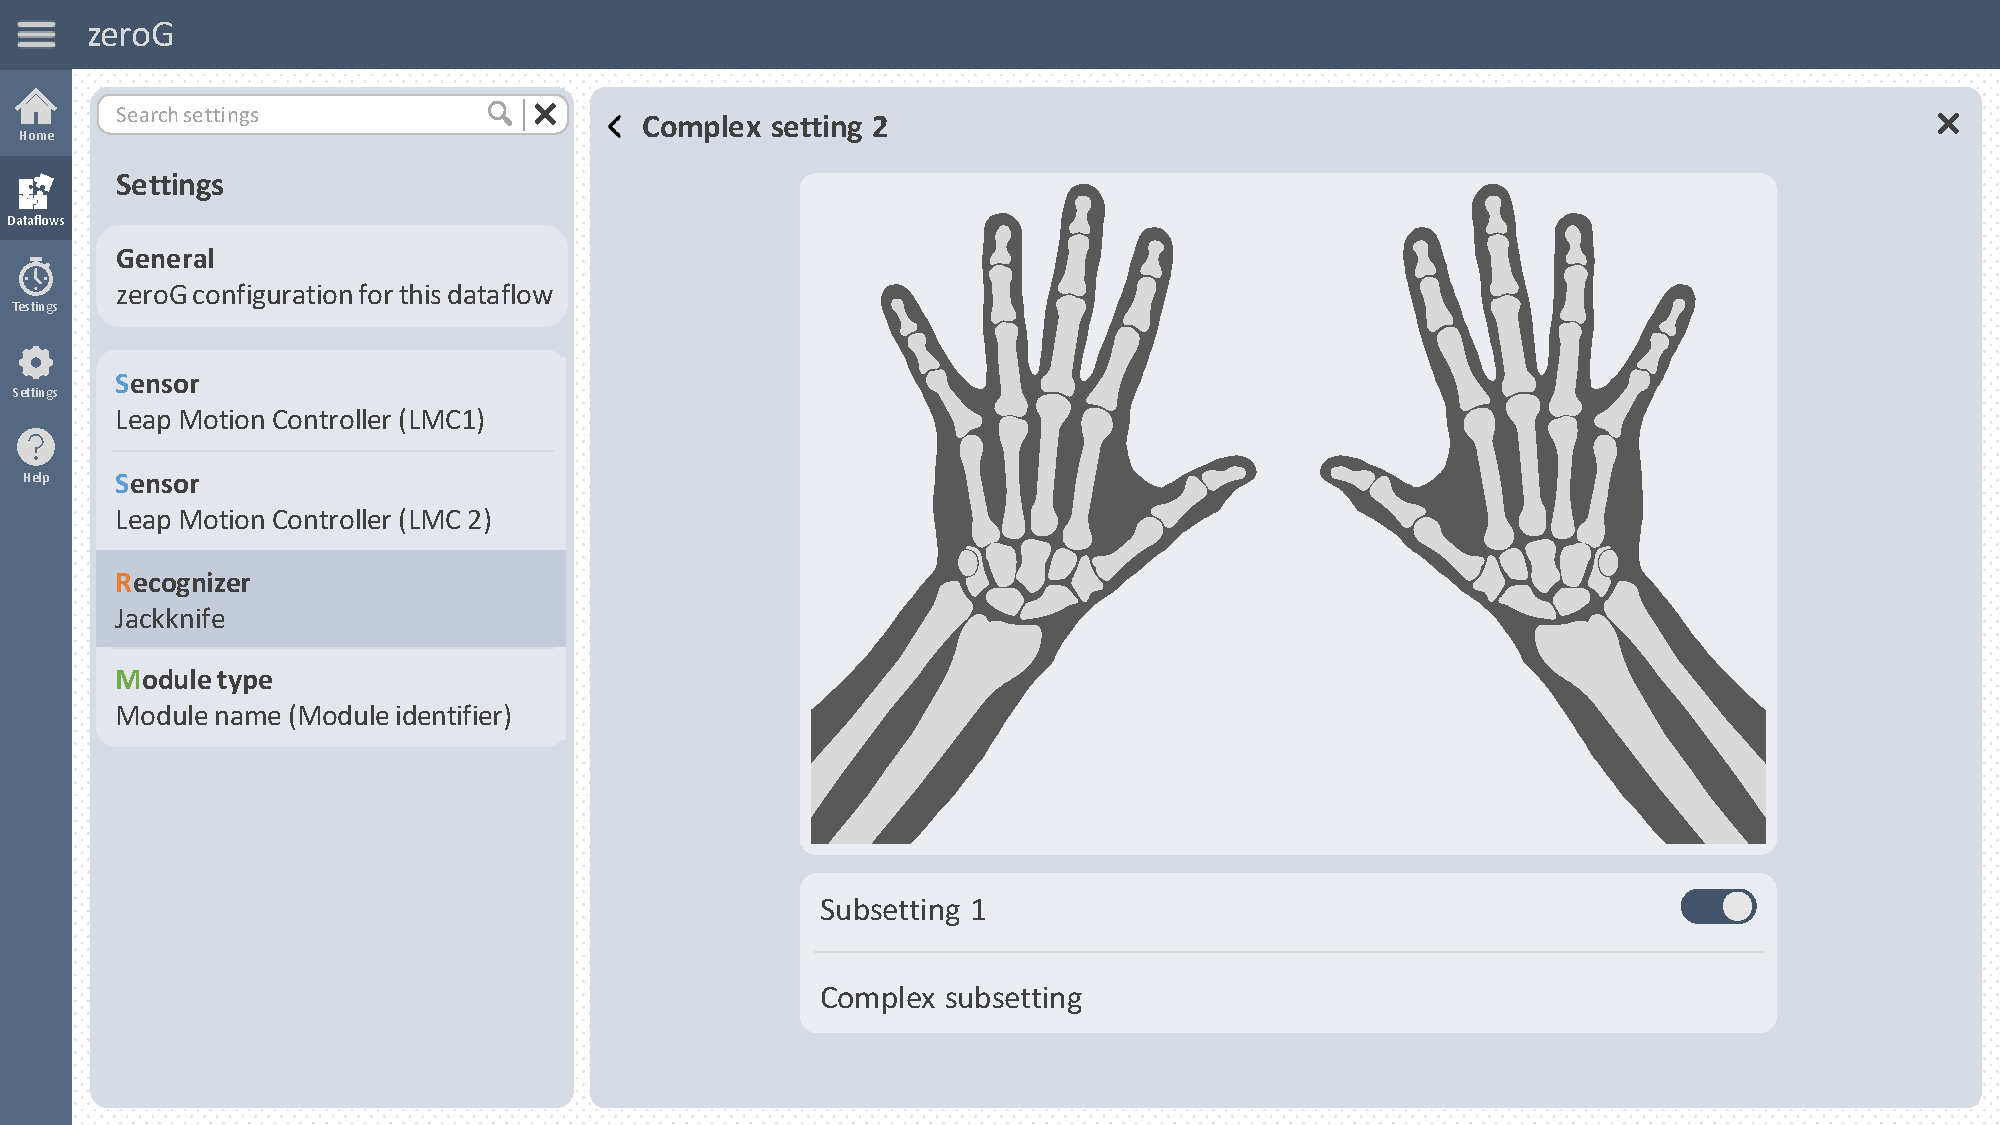
\includegraphics[width=.79\linewidth]{Figures/Conclusion/zeroG-3.pdf}  
      \vspace{-4pt}
      \captionsetup{width=.9\linewidth}
      \caption{Dataflow configuration.}
      \label{fig:zerog:ui:3}
  \end{subfigure}

  \vspace{-6pt}
  \caption{Mockups of the zeroG UI.}
  \label{fig:zerog:ui}
  % \vspace{-12pt}
\end{figure}

%% QuantumLeap Testing and Applications
Regarding tools for the development of gesture-based applications, we are currently working on a new framework for gesture recognition, named \textit{zeroG}, that aims to address the main limitations of \ql and its testing tool through profound architectural enhancements.
%
The \textit{zeroG} framework (\fig~\ref{fig:zerog:ui}) would rely on a flexible architecture based on standardized modules that could be assembled to construct complex dataflows for gesture recognition (\fig~\ref{fig:zerog:ui:2}). 
%
This architecture would cater to users of varying expertise levels: (1) experts could manually create dataflows from scratch by freely combining modules, (2) advanced users could adapt predefined dataflow templates for their applications by filling placeholders with suitable module implementations, similarly to \ql, and (3) novice users could ask \textit{zeroG} to suggest (or even generate) functioning dataflows based on some criteria like the type of application, sensor(s), and gestures.
%
Overall, the configuration GUI (\fig~\ref{fig:zerog:ui:3}) should provide ample guidance to users in the form of tutorials, tips, and module suggestions. 
%
To expedite the development process of gesture-based applications, \textit{zeroG} could generate scaffolding code to perform, among other, initialization steps like connecting to the framework and submitting a dataflow configuration.
%
In line with the \textit{compatibility} software quality property, \textit{zeroG} should seamlessly support the use of multiple applications on the same platform, without requiring user involvement. As such, it should enable applications to submit their dataflow configuration to the framework upon connection.
%
Later developments could extend to building an entire ecosystem around the framework, including databases of modules, gestures, and dataflows. This would facilitate access to components for gesture recognition and would allow \textit{zeroG} to automatically download missing components required by an application.

%% Radar pipeline
Future research could also focus on refining our pipeline for radar signal processing.
%
This includes adding some form of user normalization to account for anatomical differences between users, as well as modifying the full-wave inversion stage to take into account the finite size of the hand, thus improving gesture recognition accuracy when the distance between the user and the radar is not fixed.
% 
In addition, we could add a stage at the end of the pipeline to compute the 3D position of the hand with trilateration, which would enable applications to display a cursor on the screen, and could improve the recognition of 3D hand trajectories.
%
Similarly, we could apply sensor fusion to improve the robustness of a gesture recognition system under challenging environmental conditions.
% 
We could also investigate the possibility of recognizing gestures performed by more than one user concurrently with a single radar system and look into gesture segmentation techniques for radar to facilitate real-time gesture interaction, \eg using the \ql framework.

%% Radar experiments
Finally, future work could continue the exploration of radar-based gesture recognition through experimentation.
%
For instance, we could assess the evaluate the performance of alternative radar systems, such as phased arrays or radars featuring more spaced-out antennas, and look into the impact of radar placement (\eg on the wall, under a desk, or worn by the user) on gesture recognition.
%
We could also investigate other types of gestures, including breathing patterns (an interesting alternative to the ``sip-and-puff'' assistive technology), whole body gestures, or tongue gestures, and record them in more challenging environments, such as public spaces.
%
Additionally, we could compare the performance of Jackknife for gesture recognition with other techniques, including other template-matching algorithms and deep learning techniques, like CNNs or LSTMs.